\documentclass[12pt,a4paper]{article}
\usepackage[utf8]{inputenc}
\usepackage[spanish]{babel}
\usepackage{graphicx}
\usepackage{kpfonts}
\usepackage[left=2cm,right=2cm,top=2cm,bottom=2cm]{geometry}
\author{Jorge Bueno}
\begin{document}
\title{\textbf{Universidad Politecnica \\ de la \\ Zona Metropolitana de Guadalajara}}
\author{\textbf{Practica 9} Diagrama electrico de la interfaz de potencia\\Jorge Heriberto Bueno Gomez \\Amairani Ivette Marquez Marquez\\Ing. Mecatronica 4 B}
\maketitle
$$
\includegraphics[scale=.5]{UPCDLZMDG5783-logo.png} $$
\newpage
\section{Ojetivo} 
Controlar un Relay con un Ldr utilizando un darlington tip 112. 
Tambien controlar el circuito anterios del desarrollo del plc pero sustituyendo el 2N2222 por un TIP 112.

\section{Materiales}
\begin{tabular}{|c|}
\hline 
\textbf{Materiales }\\ 
\hline 
Fuente \\ 
\hline 
Resistencias varias\\ 
\hline 
Relay \\ 
\hline 
leds \\ 
\hline 
Cable magneto calibre 22 \\ 
\hline 
Capacitores\\
\hline 
Tip 41, Tip 42, Tip 112 \\  

\hline 
\end{tabular} 
\section{Marco teorico}
\subsection{Interfaz de potencia}
Las interfaces de potencia son dispositivos intermedios entre nuestro microcontrolador y aquellos aparatos que requieran cantidades de corriente mayores a los que pueden manejar nuestro microcontrolador (por lo general estamos hablando de 40 miliamperios como máximo por pin), motores de paso, motores DC, servomotores, lamparas incandescentes, reflectores, grupos de leds son ejemplos de dispositivos que podriamos a llegar a controlar desde el microcontrolador a través de las interfaces de potencia, es un grave error tratar de conectarlos directamente a los pines del microcontrolador. Nos valdremos de transistores, reles, puentes-H o interfaces eléctronicas de control, para construir nuestras interfaces de potencia.


\subsection{Transistores}
Los transistores pueden funcionar como amplificadores o interruptores, si los utilizamos como interruptores al igual que los relés pueden manejar corrientes altas, controlados por corrientes bajas. Los transistores son dispositivos de tres terminales (patas) y en el caso de los transistores bipolares sus terminales se llaman emisor base y colector, al poner una corriente pequeña en la base, una corriente alta puede pasar del colector al emisor. Entre los transistores bipolares podemos diferenciar dos tipos NPN y PNP.


\section{Procedimiento}
Primero analizamos el circuito a armar.\\
Despues seleccionamos los componentes a utilizar.\\
Por ultimo armamos el circuito y lo checamos.\\
\section{Resultados}
$$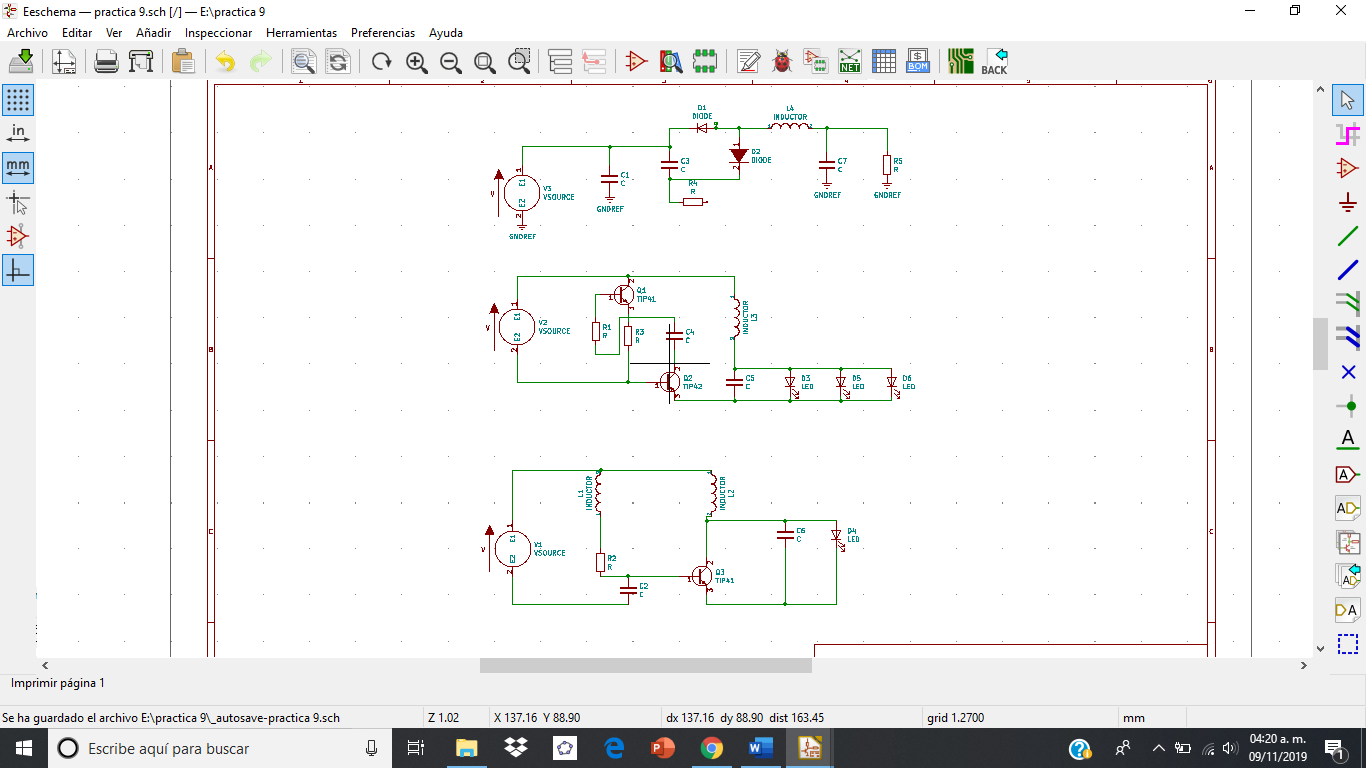
\includegraphics[scale=.3]{1.png} $$
$$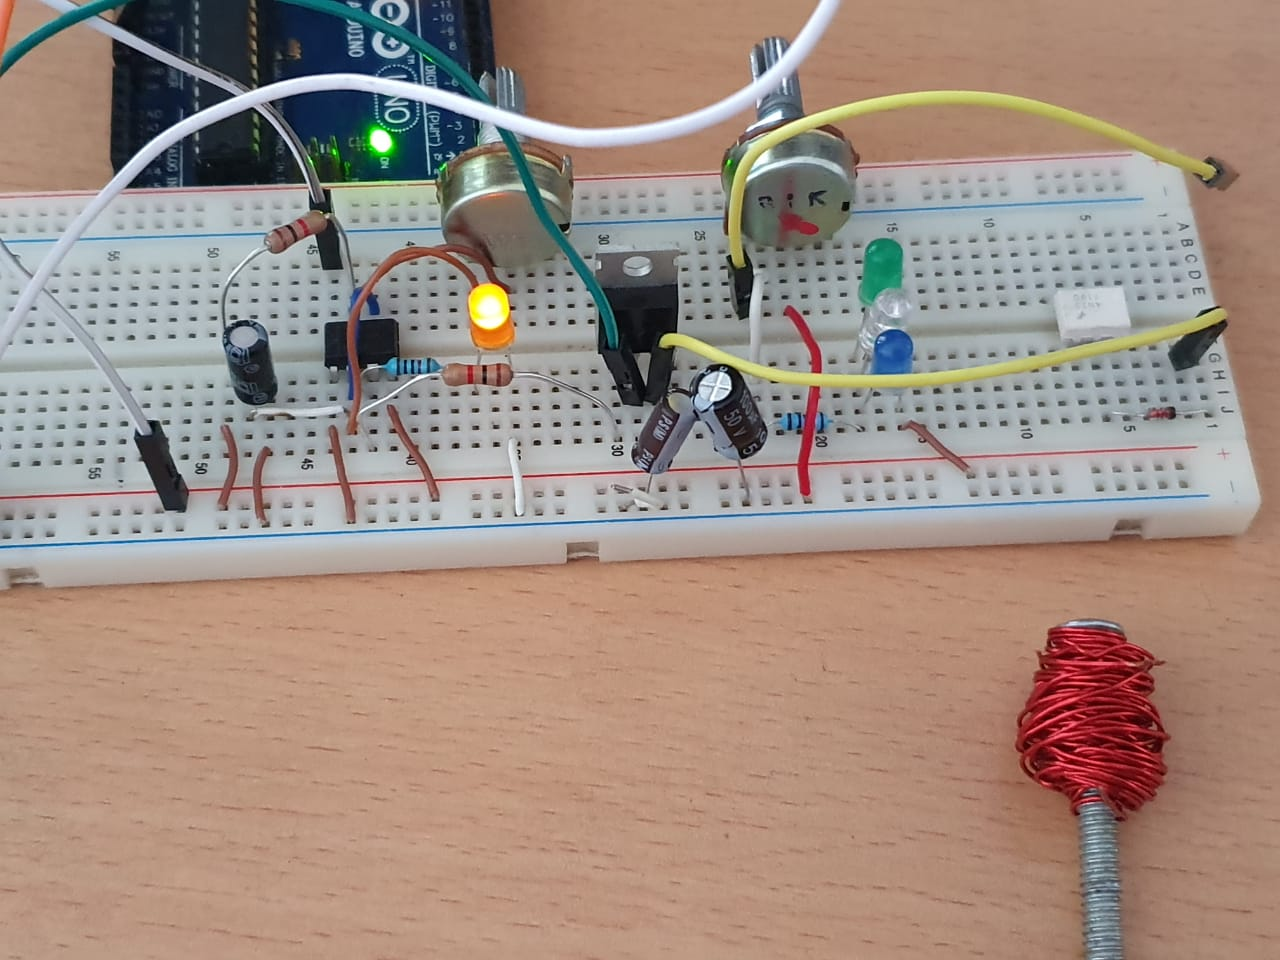
\includegraphics[scale=.3]{3.jpg} $$
\section{Conclusion}
En esta practica aprendimos al regular el voltaje mediante pulson con tres diferentes practicas, calculando el embobinado que teniamos que realizar tambien utilizanod los transistores de potencia el Tip 41 y el Tip 42, donde en un circuito tenia 12 v de entrada y esperabamos 3 de salida y o vicerveza donde le entraba 1.5 V y esperabamos 3 V de salida.
\end{document} 